\PassOptionsToPackage{unicode=true}{hyperref} % options for packages loaded elsewhere
\PassOptionsToPackage{hyphens}{url}
%
\documentclass[]{article}
\usepackage{lmodern}
\usepackage{amssymb,amsmath}
\usepackage{ifxetex,ifluatex}
\usepackage{fixltx2e} % provides \textsubscript
\ifnum 0\ifxetex 1\fi\ifluatex 1\fi=0 % if pdftex
  \usepackage[T1]{fontenc}
  \usepackage[utf8]{inputenc}
  \usepackage{textcomp} % provides euro and other symbols
\else % if luatex or xelatex
  \usepackage{unicode-math}
  \defaultfontfeatures{Ligatures=TeX,Scale=MatchLowercase}
\fi
% use upquote if available, for straight quotes in verbatim environments
\IfFileExists{upquote.sty}{\usepackage{upquote}}{}
% use microtype if available
\IfFileExists{microtype.sty}{%
\usepackage[]{microtype}
\UseMicrotypeSet[protrusion]{basicmath} % disable protrusion for tt fonts
}{}
\usepackage{hyperref}
\hypersetup{
            pdfborder={0 0 0},
            breaklinks=true}
\urlstyle{same}  % don't use monospace font for urls
\usepackage[margin=1in]{geometry}
\usepackage{longtable,booktabs}
% Fix footnotes in tables (requires footnote package)
\IfFileExists{footnote.sty}{\usepackage{footnote}\makesavenoteenv{longtable}}{}
\usepackage{graphicx,grffile}
\makeatletter
\def\maxwidth{\ifdim\Gin@nat@width>\linewidth\linewidth\else\Gin@nat@width\fi}
\def\maxheight{\ifdim\Gin@nat@height>\textheight\textheight\else\Gin@nat@height\fi}
\makeatother
% Scale images if necessary, so that they will not overflow the page
% margins by default, and it is still possible to overwrite the defaults
% using explicit options in \includegraphics[width, height, ...]{}
\setkeys{Gin}{width=\maxwidth,height=\maxheight,keepaspectratio}
\setlength{\emergencystretch}{3em}  % prevent overfull lines
\providecommand{\tightlist}{%
  \setlength{\itemsep}{0pt}\setlength{\parskip}{0pt}}
\setcounter{secnumdepth}{0}
% Redefines (sub)paragraphs to behave more like sections
\ifx\paragraph\undefined\else
\let\oldparagraph\paragraph
\renewcommand{\paragraph}[1]{\oldparagraph{#1}\mbox{}}
\fi
\ifx\subparagraph\undefined\else
\let\oldsubparagraph\subparagraph
\renewcommand{\subparagraph}[1]{\oldsubparagraph{#1}\mbox{}}
\fi

% set default figure placement to htbp
\makeatletter
\def\fps@figure{htbp}
\makeatother

\usepackage[T2A]{fontenc}
\usepackage[utf8]{inputenc}
\usepackage[russian]{babel}
\usepackage{indentfirst}
\usepackage{animate}
\usepackage{listings}
\lstset{frame=single, captionpos = b}

\author{}
\date{\vspace{-2.5em}}

\begin{document}

{
\setcounter{tocdepth}{2}
\tableofcontents
}
\begin{titlepage}
  \begin{center}
    \large
    МИНИСТЕРСТВО ОБРАЗОВАНИЯ И НАУКИ РОССИЙСКОЙ ФЕДЕРАЦИИ
    
    Федеральное агентство по образованию

    "<Пермский национальный исследовательский политехнический университет">
     
    Кафедра микропроцессорных средств автоматизации
    \vfill

    Отчёт по лабораторной работе \textnumero 2
    
    По дисциплине компьютерная графика
    
    На тему: "<Построение динамических изображений">
    
\end{center}
\vfill
 
\newlength{\ML}
\settowidth{\ML}{«\underline{\hspace{0.7cm}}» \underline{\hspace{1.5cm}}}
\hfill
\begin{minipage}{0.4\textwidth}
    Работу выполнили\\
    студенты гр. ИСУП-18-2м\\
    \underline{\hspace{\ML}} А.\,С.~Морозов\\
    \underline{\hspace{\ML}} В.\,О.~Раскошинский\\
\end{minipage}%
\bigskip
 
\hfill\begin{minipage}{0.4\textwidth}
    Проверил доцент кафедры МСА\\
    \underline{\hspace{\ML}} Л.\,А.~Мыльников\\
\end{minipage}%
\vfill
 
\begin{center}
  Пермь, 2020 г.
\end{center}
\end{titlepage}

\newpage

\hypertarget{morf}{%
\section{Алгоритм морфинга}\label{morf}}

Морфинг -- технология в компьютерной графике, визуальный эффект, создающий впечатление плавной трансформации одного объекта в другой. Встречается в трёхмерной и двумерной (как растровой, так и в векторной) графике.

Особенностью технологии морфинга является необходимость установления соответствия между точками исходного и конечного изображений.

\hypertarget{morf:rastr}{%
\section{Морфинг растровых изображений}\label{morf:rastr}}

При работе с растровыми изображениями необзодимо, чтобы разрешения исходного изображения и конечного совпадали. Тогда каждая точка исходного изображения становится в соответствие каждой точке конечного изображения, и работа алгоритма будет состоять в плавном преобразовании цвета по формуле:

\begin{equation}
  \label{morf:1}
  c = c_1 + (c_2 - c_1) \cdot t,
\end{equation}

\noindent где \(0<t<1\) -- фаза морфинга, \(c_1\) и \(c_2\) -- цвета точки первого и второго изображений. Такая операция выполняется для каждой составляющей цвета в RGB или CMYK.

Реализация алгоритма морфинга представлена в листинге \ref{code:morf:rastr}. Результаты работы алгоритма представлены на рисунке \ref{galkin}.

\begin{lstlisting}[caption = Реализация алгоритма морфинга для растровых изображений, label = code:morf:rastr]

```{.python .numberLines}
from PIL import Image
import numpy as np

im1 = Image.open('1.png')
im2 = Image.open('2.png')

while True:
    n = input("Введи число промежуточных стадий\n")
    try:
        n = int(n)
        break
    except:
        print("Число промежуточных стадий - целое число")
        continue

pix_1 = np.array(im1)
pix_2 = np.array(im2)
pix_0 = np.zeros((n,) + pix_1.shape, dtype = int)

m = np.linspace(0, 1, num = n + 2)[1:-1] # num = число картинок + 2

iint = np.vectorize(int) # векторизуем int

# алгоритм морфинга для всех промежуточных стадий
for i in range(len(m)):
    pix_0[i] = iint(iint(pix_1) + (iint(pix_2) - iint(pix_1)) * m[i])
    
pix = np.hstack((pix_1, *pix_0, pix_2)).astype(np.uint8) # массив из всех изображений
Image.fromarray(pix).show()
Image.fromarray(pix).save('gradient.png')
```
\end{lstlisting}

\begin{figure}[htb]
  \label{galkin}
  \begin{center}
      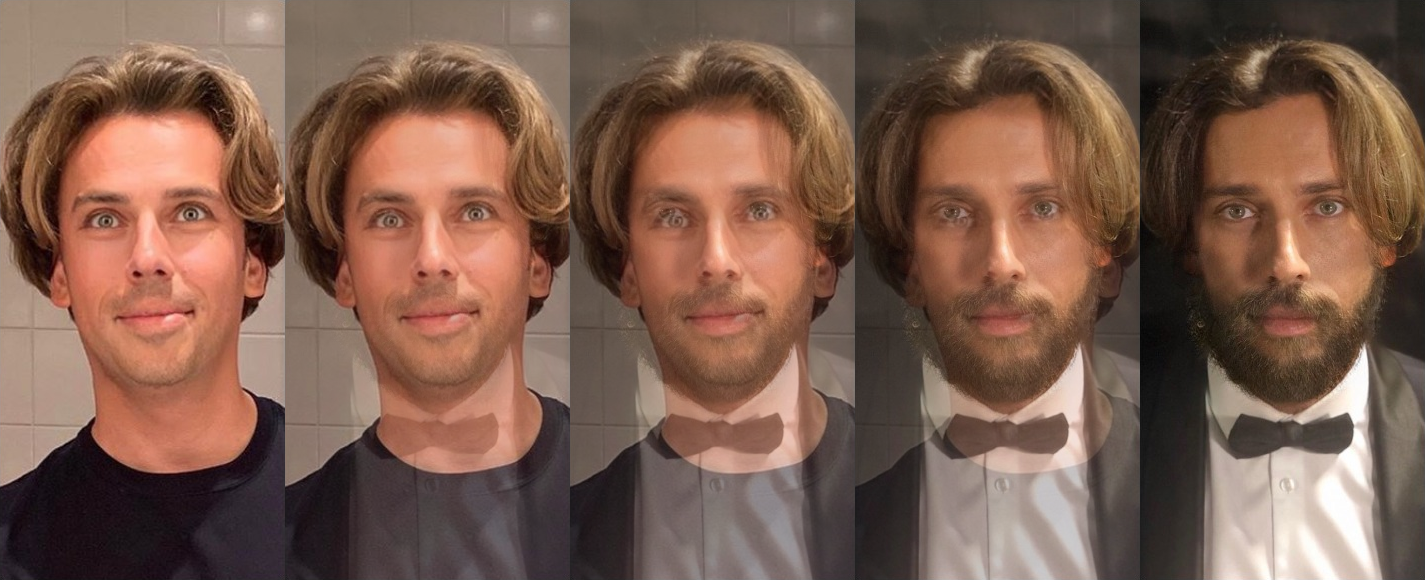
\includegraphics{../face_morphing/gradient}
  \end{center}
  \caption{Результаты работы алгоритма морфинга для растровых изображений}
\end{figure}

\hypertarget{morf:vec}{%
\section{Морфинг векторных изображений}\label{morf:vec}}

При использовании векторной графики устанавилвается соответствие между точками исходного и целевого изображения. Таким образом получаем пары значений \(\left(y_1^{(0)},x_1^{(0)}\right),\left(y_1^{(1)},x_1^{(1)}\right)\) и т.д. в зависимости от количества промежуточных состояний и точек изображений. Для изменения значений координат обычно исопльзуется уравнение прямой \((y = a + b \cdot x)\), но могут использоваться и другие фигуры, описываемые аналитически. Зная две координаты, мы можем определить значеня коэффициентов \(a\) и \(b\) из системы уравнений

\begin{center}
  \animategraphics[controls,loop,width=0.5\linewidth]{20}{../animate/frames/frame}{0}{20}
\end{center}

\end{document}
